\documentclass{article}
\usepackage[utf8]{inputenc}
\usepackage{graphicx}
\usepackage{amssymb,mathtools}   
\usepackage{tabu} 
\usepackage[
maxbibnames=99,
maxcitenames=2,
uniquelist=false,
uniquename=false,
backend=biber,
style=authoryear,
doi=false,isbn=false,url=false
]{biblatex}
\addbibresource{references.bib}
\AtEveryBibitem{%
  \clearlist{language}%
}
              
\title{Trade, migration, and the dynamics of\\ spatial interaction}
\author{Nicolas Gauthier}
\date{\small{University of Arizona}}

\begin{document}

\maketitle

\section*{Abstract}
Archaeological settlement patterns are the physical remains of complex webs of human decision-making and social interaction. Entropy-maximizing spatial interaction models are a means of building parsimonious models that average over much of this small-scale complexity, while maintaining key large-scale structural features. Dynamic social interaction models extend this approach by allowing archaeologists to explore the co-evolution of human settlement systems and the networks of interaction that drive them. Yet, such models are often imprecise, relying on generalized notions of settlement ``influence'' and ``attractiveness'' rather than concrete material flows of goods and people. Here, I present a disaggregated spatial interaction model that explicitly resolves trade and migration flows and their combined influence on settlement growth and decline. I explore how the balance of costs and benefits of each type of interaction influence long-term settlement patterns. I find trade flows are the strongest determinant of equilibrium settlement structure, and that migration flows play a more transient role in balancing site hierarchies. This model illustrates how the broad toolkit for spatial interaction modeling developed in geography and economics can increase the precision of quantitative theory building in archaeology, and provides a road-map for connecting mechanistic models to the empirical archaeological record.

\section{Introduction}

Regional archaeological settlement patterns arise from the interactions of many individual agents, each making decisions with imperfect and incomplete information about the costs and benefits of social interaction. Yet, in spite of this complexity at the individual scale, empirical regularities emerge at larger scales. So-called ``entropy-maximizing'' spatial interaction models capitalize on this change-of-scale property. Entropy maximization is a means of estimating the large-scale properties of a system by making the fewest possible assumptions about micro-scale dynamics \parencite{Presse2013, Thurner2017ThePrinciple}. Entropy here is a measure of micro-scale uncertainty, and maximizing it reveals the most probable macro-scale system configuration. An entropy-maximizing spatial interaction model estimates the large-scale \emph{flows} of a constrained quantity, such as goods and people, between discrete spatial zones as a function of their distance and their mutual ``attractiveness'' \parencite{Wilson1971a}. It works by systematizing the basic costs and benefits used in decision-making and scaling them up ensuring that simple self-consistency constraints (such as total inflows equals total outflows) are met. 

Archaeologists have embraced this modeling paradigm to infer past human behaviors from the pattern of settlements visible on the landscape. Archaeologists have successfully used these models to assess the sensitivity of estimated settlement structures to uncertainty in the archaeological record \parencite{Bevan2013, Paliou2016}, model the evolution of site hierarchies absent top-down forces \parencite{Altaweel2015}, explore the role of historical contingency in the development of major settlements \parencite{Evans2017WasNecessary}, and determine key factors in the formation known urban networks in varying locations and time periods \parencite{Davies2014, Altaweel2015a, Palmisano2015, Filet2017}.

In isolation, an entropy-maximizing interaction model is essentially a statistical tool, estimating the most likely configuration of flows between settlements given the relevant constraints. \emph{Dynamic} spatial interaction models, on the other hand, combine these flow estimates with one or more mechanistic models to describe how the flows wax and wane over time \parencite{Harris1978}. In such cases, the spatial interaction model captures the ``fast'' dynamics -- the balance of flows between locations as a function of their relative size or importance -- and the mechanistic model captures the ``slow'' dynamics governing how the locations grow or decline because of their access to those flows. As implemented in archaeology, the slow dynamics are typically equilibrium-seeking and settlements evolve only to balance inflows and outflows. As a result, many archaeological applications of these models use them as heuristic tools for finding equilibrium settlement distributions rather than as dynamical models that explicitly resolve the time evolution of settlement systems \parencite{Bevan2013}. 

Powerful alternatives to the equilibrium-seeking slow dynamic in archaeological spatial interaction models are Lotka-Volterra consumer resource equations. Lotka-Volterra equations are used in ecology to model energy flows in a food web. More generally, these models can represent energy flows in any social-ecological system, such as an agricultural settlement consuming resources from its hinterland \parencite{Anderies2011a, Qubbaj2014}. Spatial interaction models are particularly useful for incorporating spatial richness into Lotka-Volterra models, which would otherwise resolve space only implicitly \parencite{Wilson2006}. Models that use entropy maximization to estimate the ``fast'' flow dynamics and consumer-resource equations to represent the ``slow'' settlement dynamics are known as Boltzmann-Lotka-Volterra models \parencite{Wilson2008}. These systems of equations are able to capture the dynamic feedbacks between settlements and the networks connecting them. 

In order to keep them flexible, archaeological spatial interaction models are typically abstract and highly aggregated. The flows are assumed to be some aggregate of trade and migration reflecting the ``influence'' of each site on another, and the settlement state variable that evolves in time is some generalized notion of ``attractiveness.'' While these generalizations are useful for empirical work, they elide much of the processual granularity that makes these models such a useful tool for quantitative theory building. Metabolic costs, such as the energy expended producing and transporting food over space where transportation infrastructure is sparse, provide constraints on energy flows in exchange systems \parencite{Drennan1984,Verhagen2019ModellingApproaches}. In any particular case, the balance between these costs and the metabolic benefits of social interaction influences whether resources are moved in bulk to populations in a settlement or whether those populations move themselves to the available resources. In order to determine how the balance of these flows influence long-run settlement patterns it is thus necessary to replace the generalized notion of flows of ``influence'' with more direct estimates of trade and migration flows and a more concrete mechanistic model for how these flows influence settlement dynamics.

Here, I present a dynamic spatial interaction model that explicitly tracks the flows of trade and migration within a settlement system. I use a variant of the Lotka-Volterra equations known as a ``competition for resources'' model, in which a population of urban settlements competes for access to food from multiple agricultural resource patches. The populations of these settlements grow and decline according to the flow of resources into the settlements and the flow of migrants between them. Using a disaggregated, two-part spatial interaction model, I model the flows of food to people (``trade'') and the flows of people to food (``migration'') separately and explore how varying the relative costs of each type of movement influences the resulting population distribution at equilibrium. I show that the constraint on moving food to people is the primary determinant of long-run settlement patterns, shaping the extractive reach of settlements and their ultimate carrying capacity. Migration costs play a secondary role enhancing or diminishing existing settlement hierarchies depending on the specific migrant objectives. These findings contribute to the ongoing development of quantitative theory of spatial interaction in premodern societies, but also provide important caveats for interpreting statistical analyses of archaeological networks.

\section{Methods}

\subsection{Population Growth and Decay: The ``Slow'' Dynamics}

I explore a simple model of agricultural settlements in a patchy environment. The basic unit is a settlement, representing any urban or semi-urban population in an agricultural society consuming food from resource patches to support a population of non-farmers. The dynamics of food production are left external to the model, and it is assumed that a fixed volume of food resources are produced each year. The core dynamic of the urban population is represented as

\begin{equation} 
  \dot{N} = rN,
  \label{eq:growth1}
\end{equation}

where $\dot{N}$ is the time rate of change of population $N$ and $r$ is the realized growth rate. The realized growth rate depends on the resource consumption of $N$ as

\begin{equation} 
  r =
  \begin{cases} 
      \epsilon \left(X -  N \right) & \text{if } \epsilon \left(X - N\right) < r_{\mathit{max}} \\
      r_{\mathit{max}} & \text{otherwise},\\
   \end{cases}
   \label{eq:rate}
\end{equation}
where $X$ is the amount of available resources, $\epsilon$ is a parameter that controls the rate at which the resource surplus increases or decreases the population, and $r_{\mathit{max}}$ is the maximum growth rate. This equation states that the population grows or shrinks in proportion to its consumption of resources, but it cannot grow faster than a biological maximum rate. For simplicity, assume that $X$ is scaled to units of $N$ so that one unit of resource is sufficient to maintain one unit of population. The resulting process is a hybrid of exponential and logistic growth, with the population growing quickly when consumption is far above population and more gradually when consumption is close to the current needs of the population (i.e. ``carrying capacity'') (Figure \ref{fig:growth-models}).

\begin{figure}
    \centering
    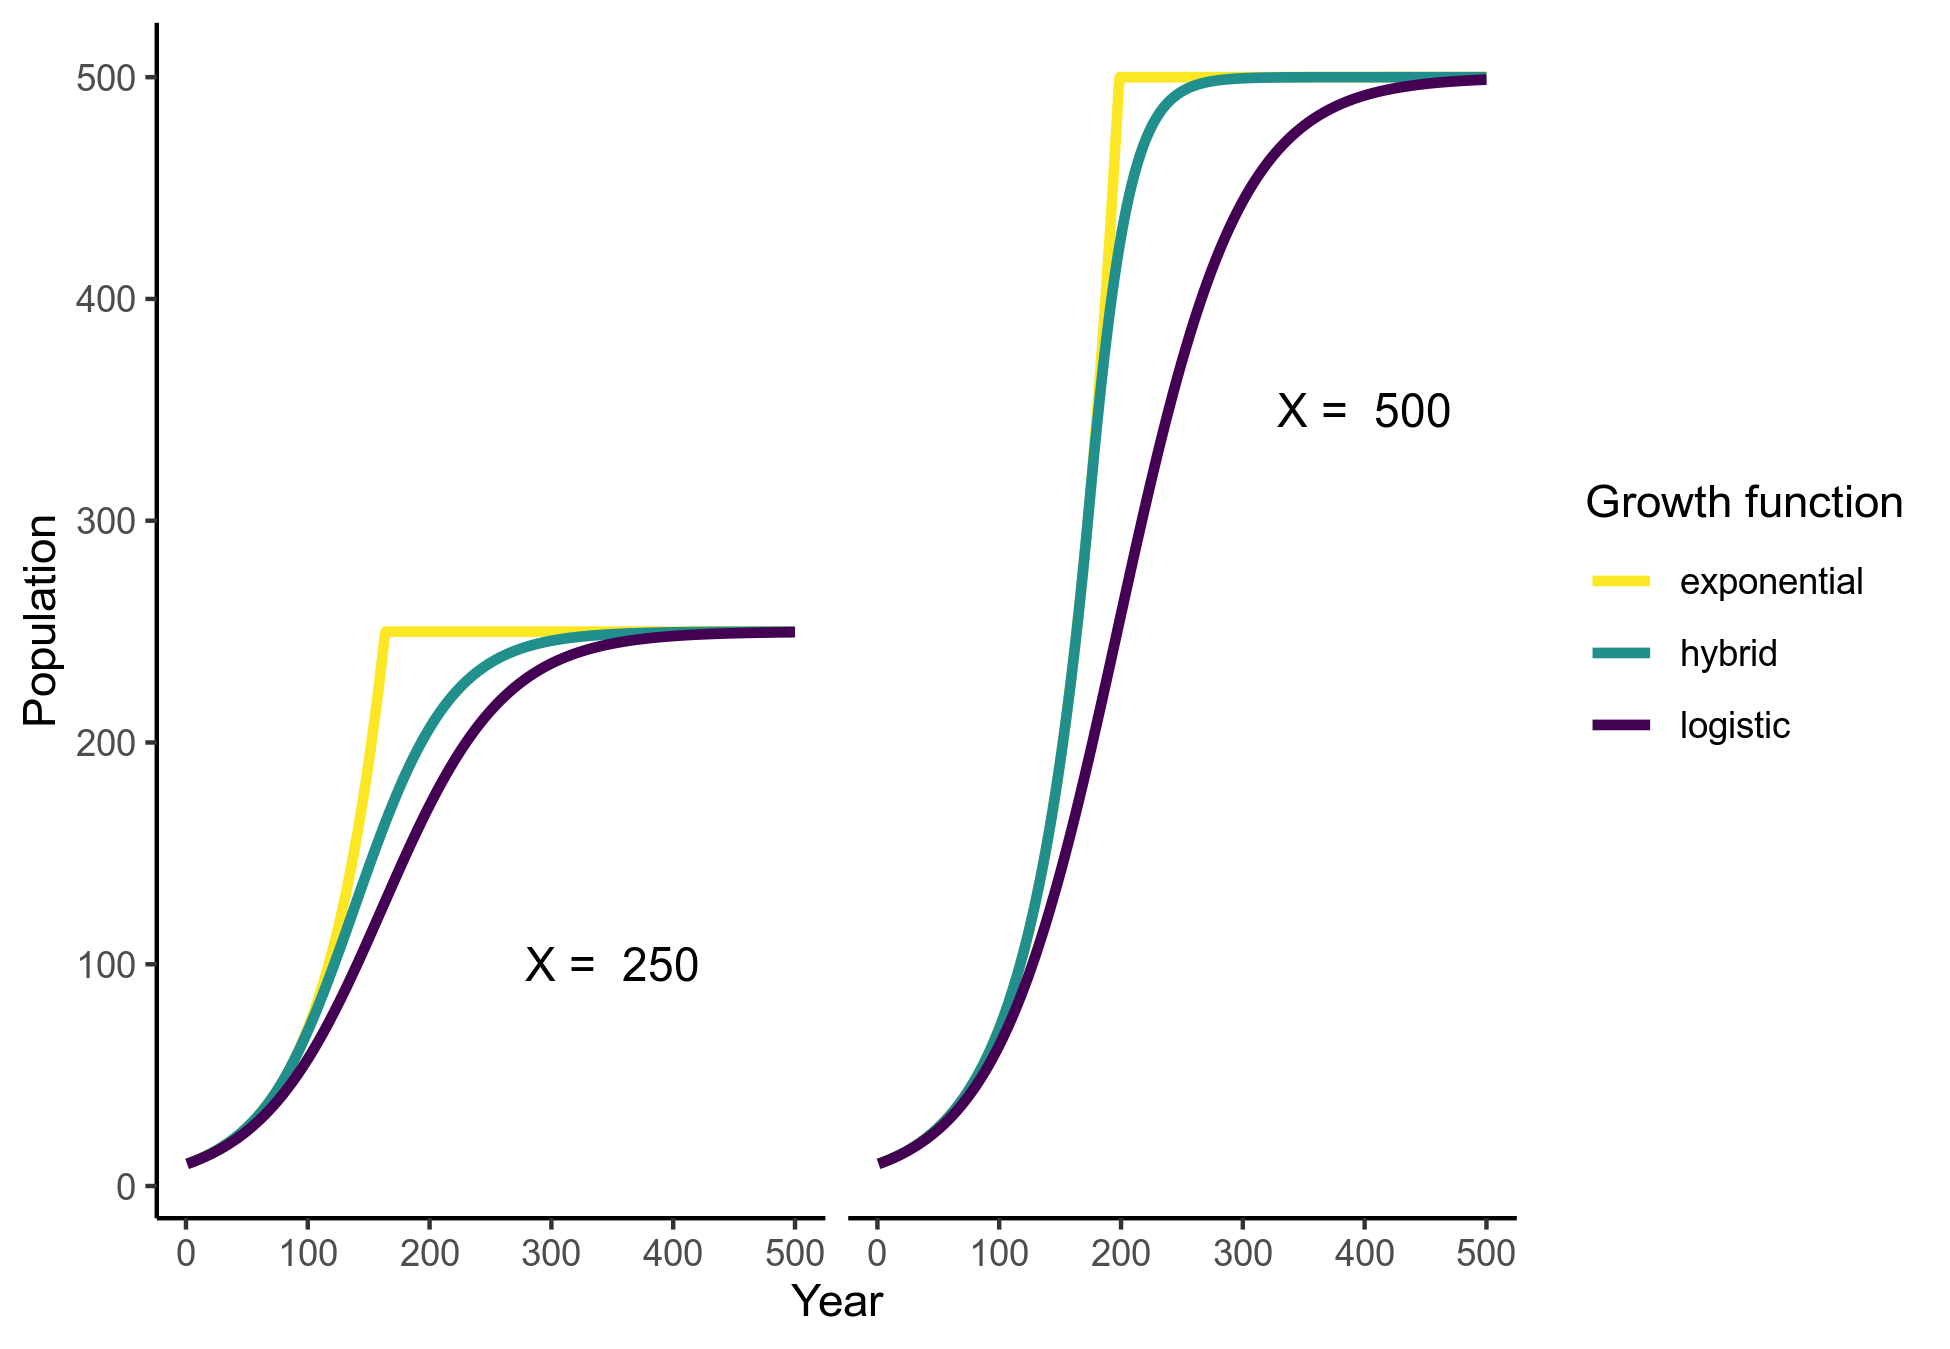
\includegraphics[width=\columnwidth]{images/growth-models.png}
    \caption[Simulations from the growth model, compared to exponential and logistic growth for two levels of resources]{Simulations from the growth model, compared to exponential and logistic growth for two levels of resource surplus $X$ over the same time span. $X$ acts as a carrying capacity. When $X$ is low, the potential for growth is low and the population approaches carrying capacity gradually similar to logistic growth. When $X$ is far above $N$ the population exponentially, with growth rates only declining shortly before carrying capacity is reached.}
    \label{fig:growth-models}
\end{figure}

Rather than a single settlement-resource system, the model represents a network of hundreds of interacting settlements and resource patches (Figure \ref{fig:spatial-domain}). The landscape is discretized into hexagonal resource patches with radius 5km, over which settlements are uniformly distributed. Settlements compete with one another for the fixed resources produced in each patch each time step, a dynamic analogous to the ``competition for resources'' model common in ecology. Not only do settlements interact indirectly with one another by harvesting the same patch, but they interact directly by exchanging population through migration. Each model year, a fixed proportion of a settlement's population leaves each city. These migrants select their destination based on the size and distance of potential migration destinations (including their origin location) and the relative \emph{per capita} resource extraction rate of each settlement.

\begin{figure}
    \centering
    
\includegraphics[width=.7\columnwidth]{images/spatial-domain.png}
    \caption[Spatial domain for the simulation experiments]{Spatial domain for the simulation experiments. The resource patches are 300 evenly-sized hexagons with radius 5km arranged in a continuous tiling with a total size of approximately 19,500 km2. Settlements are arranged in a triangular lattice located at the centroids of each hexagonal patch, and are connected by a system of physical paths joining each settlement to its six nearest neighbors.}
    \label{fig:spatial-domain}
\end{figure}

The simple mathematical model presented above can thus be extended into a social-ecological network of multiple interconnected consumer-resource systems. First, disaggregate $X$ and $N$ into $X_i$ and $N_j$, representing the resources at location $i$ and the population at location $j$. Then, introduce two flow matrices $\mathbf{T}$ and $\mathbf{M}$ that represent trade and migration flows, respectively, such that the volume of resources produced in patch $X_i$ that are consumed by the population in settlement $N_j$ is $T_{ij}$, and the number of migrants moving from settlement $N_i$ to $N_j$ is $M_{ij}$. For simplicity, the harvest of resources from patches is referred to as ``trade'', although it generally reflects any movement of food from one location to a population center in another, including non-market forms of exchange such as sharing, exchange, or tribute. Assuming a \emph{per capita} out migration rate of of $\nu$, the expanded version of Eq. \ref{eq:growth1} and \ref{eq:rate} is thus:

\begin{equation}
\dot{N_j} = rN_j - \nu N_j + \sum_i M_{ij},
\label{eq:growth2}
\end{equation}

\begin{equation}
r =
  \begin{cases} 
      \epsilon \left(\sum_i T_{ij} -  N_j \right) & \text{if }\epsilon \left(\sum_i T_{ij} -  N_j\right) < r_{\mathit{max}} \\
      r_{\mathit{max}} & \text{otherwise}.\\
   \end{cases}
\end{equation}

Together, these equations state that the population of each settlement grows according to the total inflow of resources from every patch and the total inflow of migrants from every settlement. Because all settlements compete for resources from every patch and compete with each other for migrants, the growth of one settlement depends in part on that of all other settlements. Next, I show how the resource and migrant flows represented in $\mathbf{T}$ and $\mathbf{M}$ themselves emerge from these population dynamics.

\subsection{Trade, Migration, and Spatial Interaction: The ``Fast'' Dynamics}

The model tracks two kinds of spatial flow using separate spatial interaction models: movement of resources from patches into settlements and movement of people between settlements. Both cases use similar ``production-constrained'' spatial interaction models. The general approach, first used in archaeology by \textcite{Rihll1991}, takes a fixed volume of flow ``produced'' at each location and allocates it among all potential destinations in proportion to the relative costs and benefits of interacting with each. Benefits are assessed as a power function of one or more settlement-level variables (such as size) that attract flows, and costs are assessed as a negative exponential function of distance (Figure \ref{fig:functions}). Two parameters, $\alpha$ and $\beta$, control the strength of these influences. When $\alpha > 1$ the benefits of interaction exhibit increasing returns to scale. $\beta$ is in units of distance, and can be interpreted as the distance at which the strength of interaction decays to about two-thirds of its original value.

\begin{figure}
    \centering
    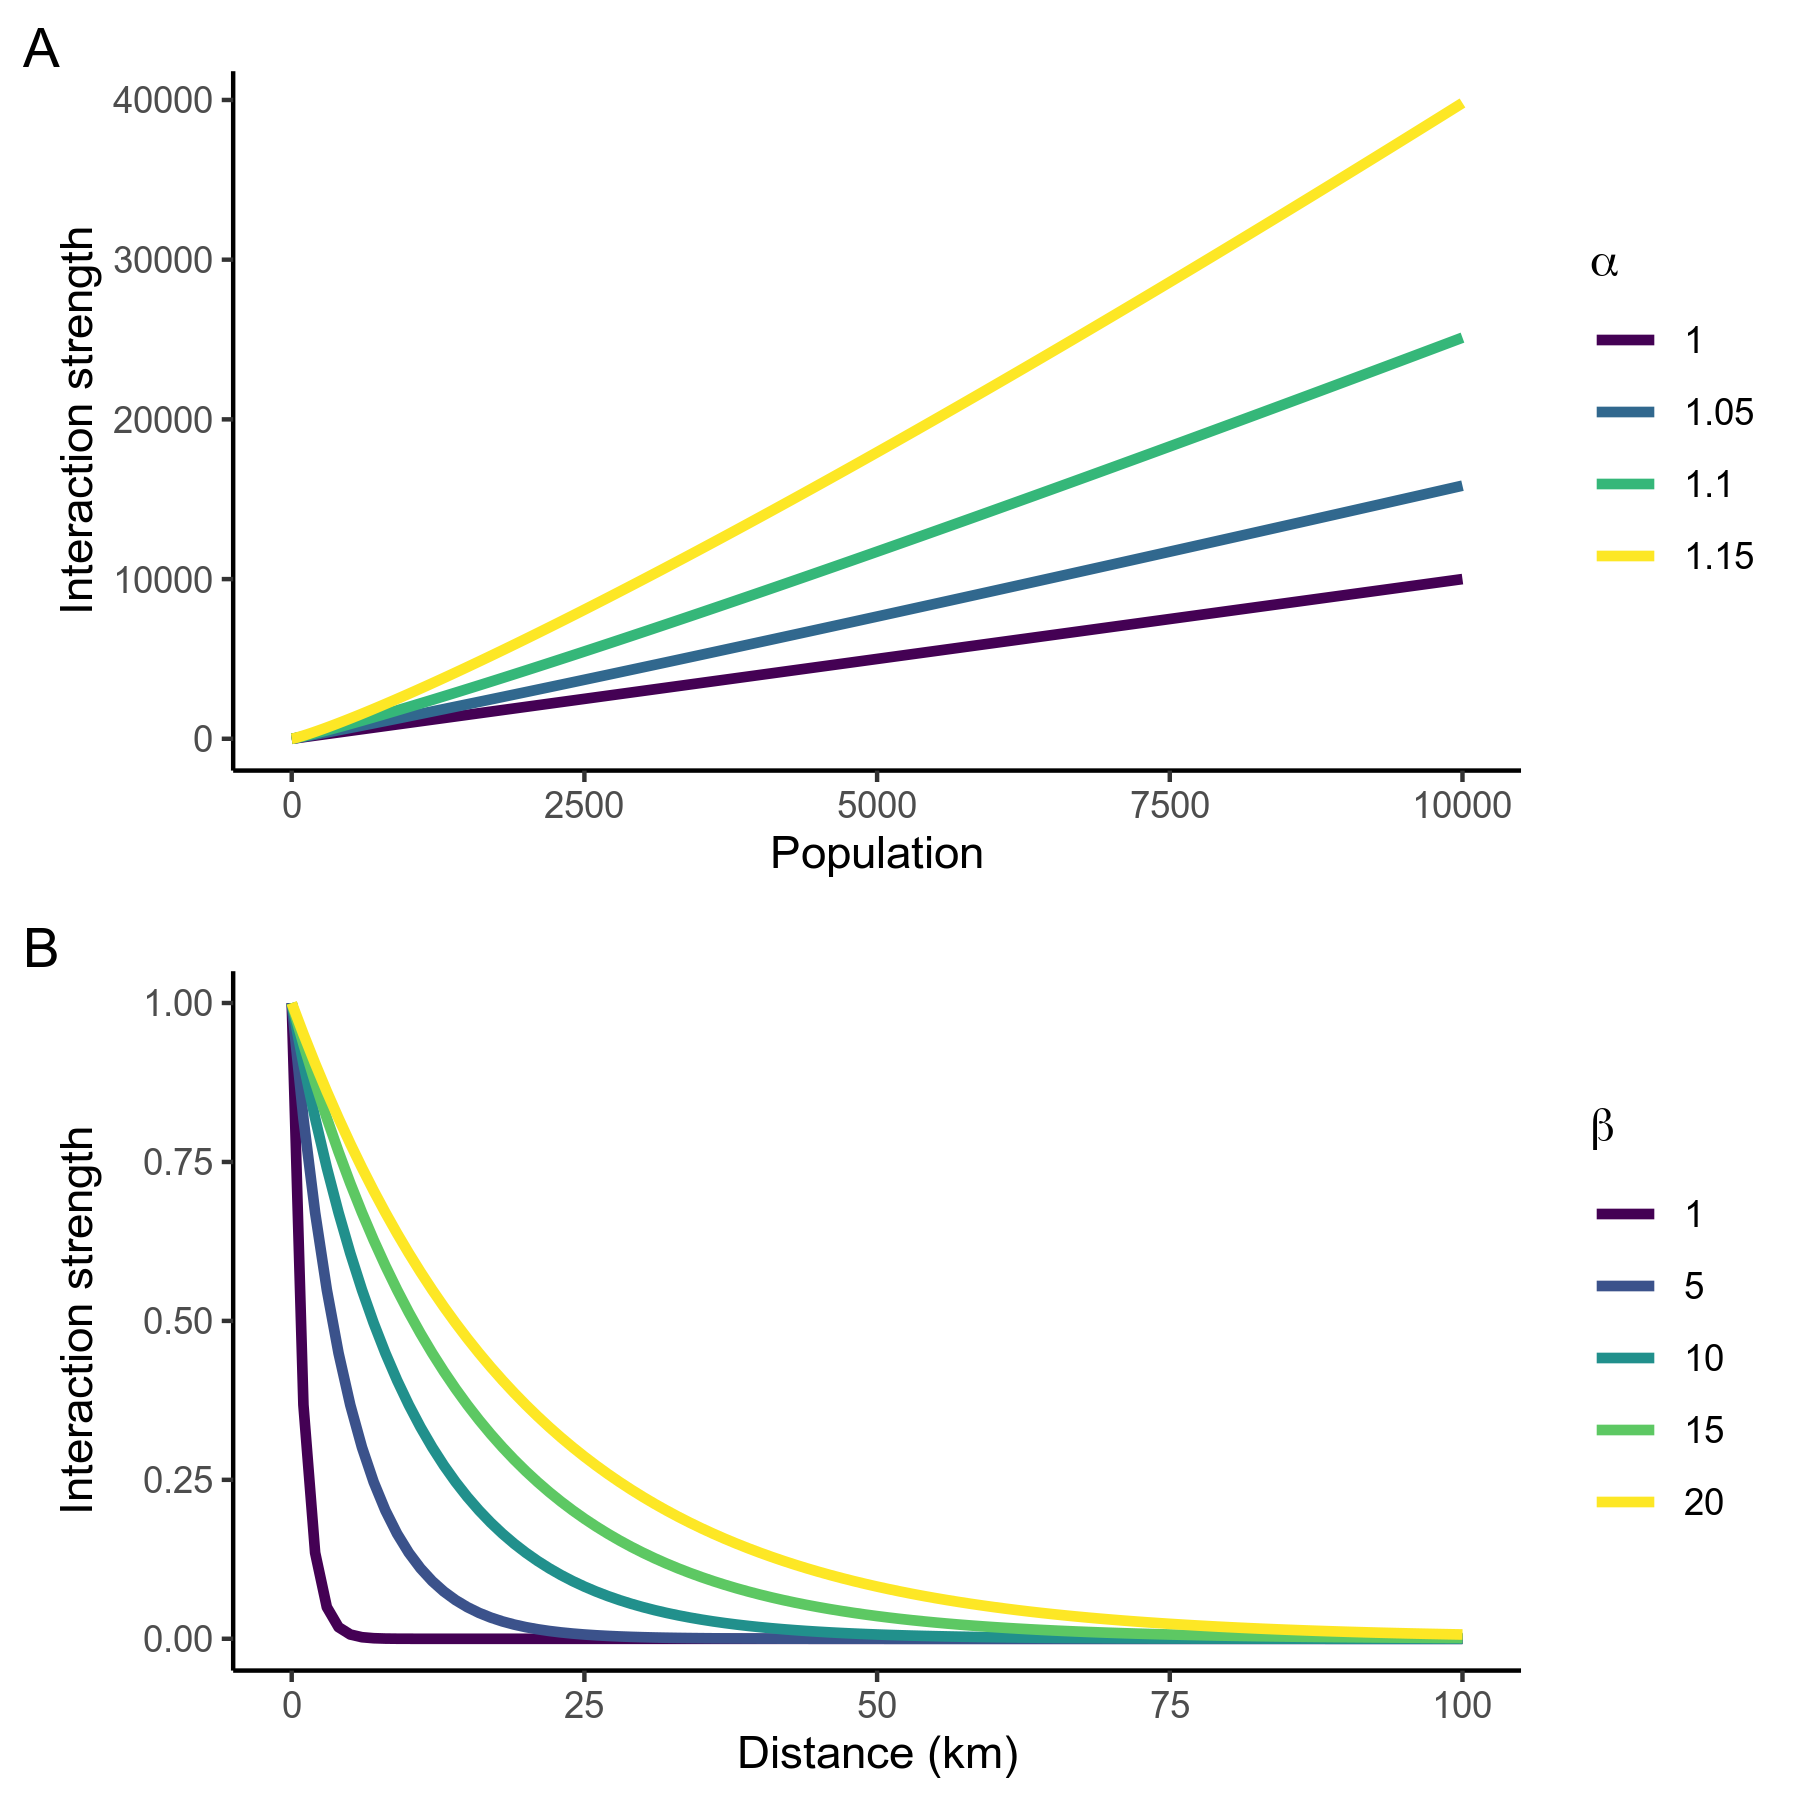
\includegraphics[width=\columnwidth]{images/functions.png}
    \caption[Functional forms for the spatial interaction models]{Functional forms for the spatial interaction models. A) Settlement-level variables influence the attractiveness of each settlement via a power function, with the parameter $\alpha$ governing the importance of that variable. B) The costs of moving over space take the form of a negative exponential function, with the parameter $\beta$ determining the steepness of the falloff of interaction with distance (higher values of $\beta$ allow interaction to occur at farther distances).}
    \label{fig:functions}
\end{figure}

The spatial interaction model for trade is a simple ``gravity'' model, in which settlement population $N$ is the only variable determining a settlement's attractiveness. Thus the flow of resources from patch $i$ to settlement $j$, is

\begin{equation}
    T_{ij} =  X_i  \frac{N_j^{\alpha_1} \exp\left(-c_{ij} / \beta_1 \right)}{ \sum_k N_k ^ {\alpha_1} \exp \left( -c_{ik} / \beta_1 \right)},
    \label{eq:trade}
\end{equation}
where $X_i$ is the amount of resources produced in the patch -- the ``production'' term that is ``constrained'' in the model -- and $c_{ij}$ is the cost of moving from $i$ to $j$ (distance in kilometers). The terms in the fraction simply assess the relative costs and benefits, with the numerator representing the utility of moving food to settlement $i$ and the denominator the sum of the utilities for all potential destination locations, together ensuring that the total outflows equal the total resources in $X_i$. Because of this balancing factor, all trade flows among settlements can be computed simultaneously and there is no need to evaluate the flows to each settlement sequentially. A settlement has no special access to its local resource patch, save only for its proximity relative to other settlements ($c_{ij} = 0 \text{ if } i = j$).

The migration flows depend in part on the trade flows, and are modeled in a similar fashion. The number of migrants moving from settlement $i$ to $j$ is 

\begin{equation}
  M_{ij} =  \nu N_i \frac{N_j^{\alpha_1} W_j^{\alpha_2} \exp\left(-c_{ij} / \beta_2 \right)}{ \sum_k N_k^{\alpha_1}  W_k^{\alpha_2} \exp \left( -c_{ik} / \beta_2 \right)},
  \label{eq:migration}
\end{equation}
where $\nu N_i$ is the number of migrants originating in $i$ and $W_j = \sum_iT_{ij}/N_j$ is the \emph{per capita} welfare of $j$, defined as the ratio of trade inflows to population. As with trade, all migrant flows occur simultaneously in a time step due to the production constraint term, and after all trade flows are computed. Unlike in the trade equation (\ref{eq:trade}), the attractiveness of a given settlement as a migration destination depends on both its population size and its welfare. Migrants will thus seek out destinations with lots of well-fed people, and the relative values of $\alpha_1$ and $\alpha_2$ determine the relative importance of each factor.

In summary, the flow of resources from each resource patch to each settlement is first determined by Equation \ref{eq:trade}, which depends on the underlying distribution of resources and settlement populations. Then, the flow of migrants between settlements is determined by Equation \ref{eq:migration}, based on the settlement populations and the flow of resources. Finally, the populations of the settlements grow both by consuming trade resources and by accepting new migrants according to Equation \ref{eq:growth2}, and this new population distribution will feed back to influence future trade and migrant flows. The entire system is a complicated web of nonlinear interaction, as the growth and decline of settlements can potentially depend on all other settlements. The complexity of this system increases geometrically as the number of settlements increases, precluding exact analytic solutions. We must instead leverage numerical simulations to capture these complex spatial interactions.

\section{Analysis}

The disaggregated spatial interaction model was run from uniform initial conditions, with $X = 200$ and $N = 25$, for 2000 years or until the system reached an equilibrium. This analysis focuses on the behavior of system under different combinations of the parameters that control the costs and benefits of interaction $\alpha_1, \alpha_2, \beta_1, \beta_2$. The parameter $\alpha_1$ determines how the population size of a settlement influences its attractiveness as a target for trade and migration, and $\alpha_2$ determines how this attractiveness depends on \emph{per capita} welfare. $\beta_1$ and $\beta_2$ both correspond to units of distance (here kilometers) and determine the impact of distance on the intensity of flows, with the former representing the ease of moving resources to population centers and the latter the ease of moving people among population centers. Settlement patterns under different parameterizations were assessed via graphical comparison and statistical analysis of aggregate quantities including the total population, count of settlements, and an index of population dispersion and concentration. The following analysis focuses on the area of the parameter space where $\alpha_{1,2} \geq 1$ and $\beta_1 \leq \beta_2$, reflecting assumptions that there are positive returns to scale in attractiveness and that moving people over the landscape is easier than moving bulk food supplies. 


\begin{table}[h] % Table float
\begin{center}
    
\caption{Parameters, their default values, and ranges explored.}
\label{table1}
\begin{tabu}{l c c} \\ \hline
    Parameter & Value & Interpretation \\ \hline
    $\epsilon$ & 0.0001 & Consumption adjustment rate \\   
    $r_{\mathit{max}}$ & 0.02 & Maximum growth rate \\
    $\nu$ & 0.05 & Migration rate \\
    $\alpha_1$ & [1.0, 1.05, 1.1, 1.15]   &  Returns to population size \\
    $\alpha_2$ & [0, 1.0, 1.05, 1.1, 1.15] & Returns to \textit{per capita} welfare \\
    $\beta_1$ & [5, 10, 15, 20] & Ease of moving food to people  \\
    $\beta_2$ & [5, 10, 15, 20]   &    Ease of moving people to food \\ \hline
\end{tabu}
\end{center}
\end{table}

\subsection{The Movement of Food to People Defines Settlement Territory Size, Migration Costs Mediate the Distribution of Population}

How does the cost of moving food and people over distance, as encoded in the $\beta$ parameters, influence settlement patterns at equilibrium? The $\beta$ parameters are the primary way space is introduced into the model. By design, the costs of moving food and other resources from resource patches to settlements will be different from the costs of moving people between settlements. The balance of these cost factors can introduce complexity into the spatial patterns that result from these interactions. 

For cases where migration is based only on population size, not welfare ($\alpha_1 = 1.15, \alpha_2 = 0$), increasing $\beta_1$ to allow food to be moved longer distances to reach settlements decreases the number of inhabited settlements and increases their size at equilibrium (Figure \ref{fig:beta1}a). As the number of settlements at equilibrium decreases, these major settlements also move closer to the center of the domain, corresponding to the locations with the maximum access to resources given the travel costs. This competition for resource access can be visualized by connecting each resource patch to the settlement to which the majority of its resources travel  (Figure \ref{fig:beta1}b). 

\begin{figure}
    \centering
    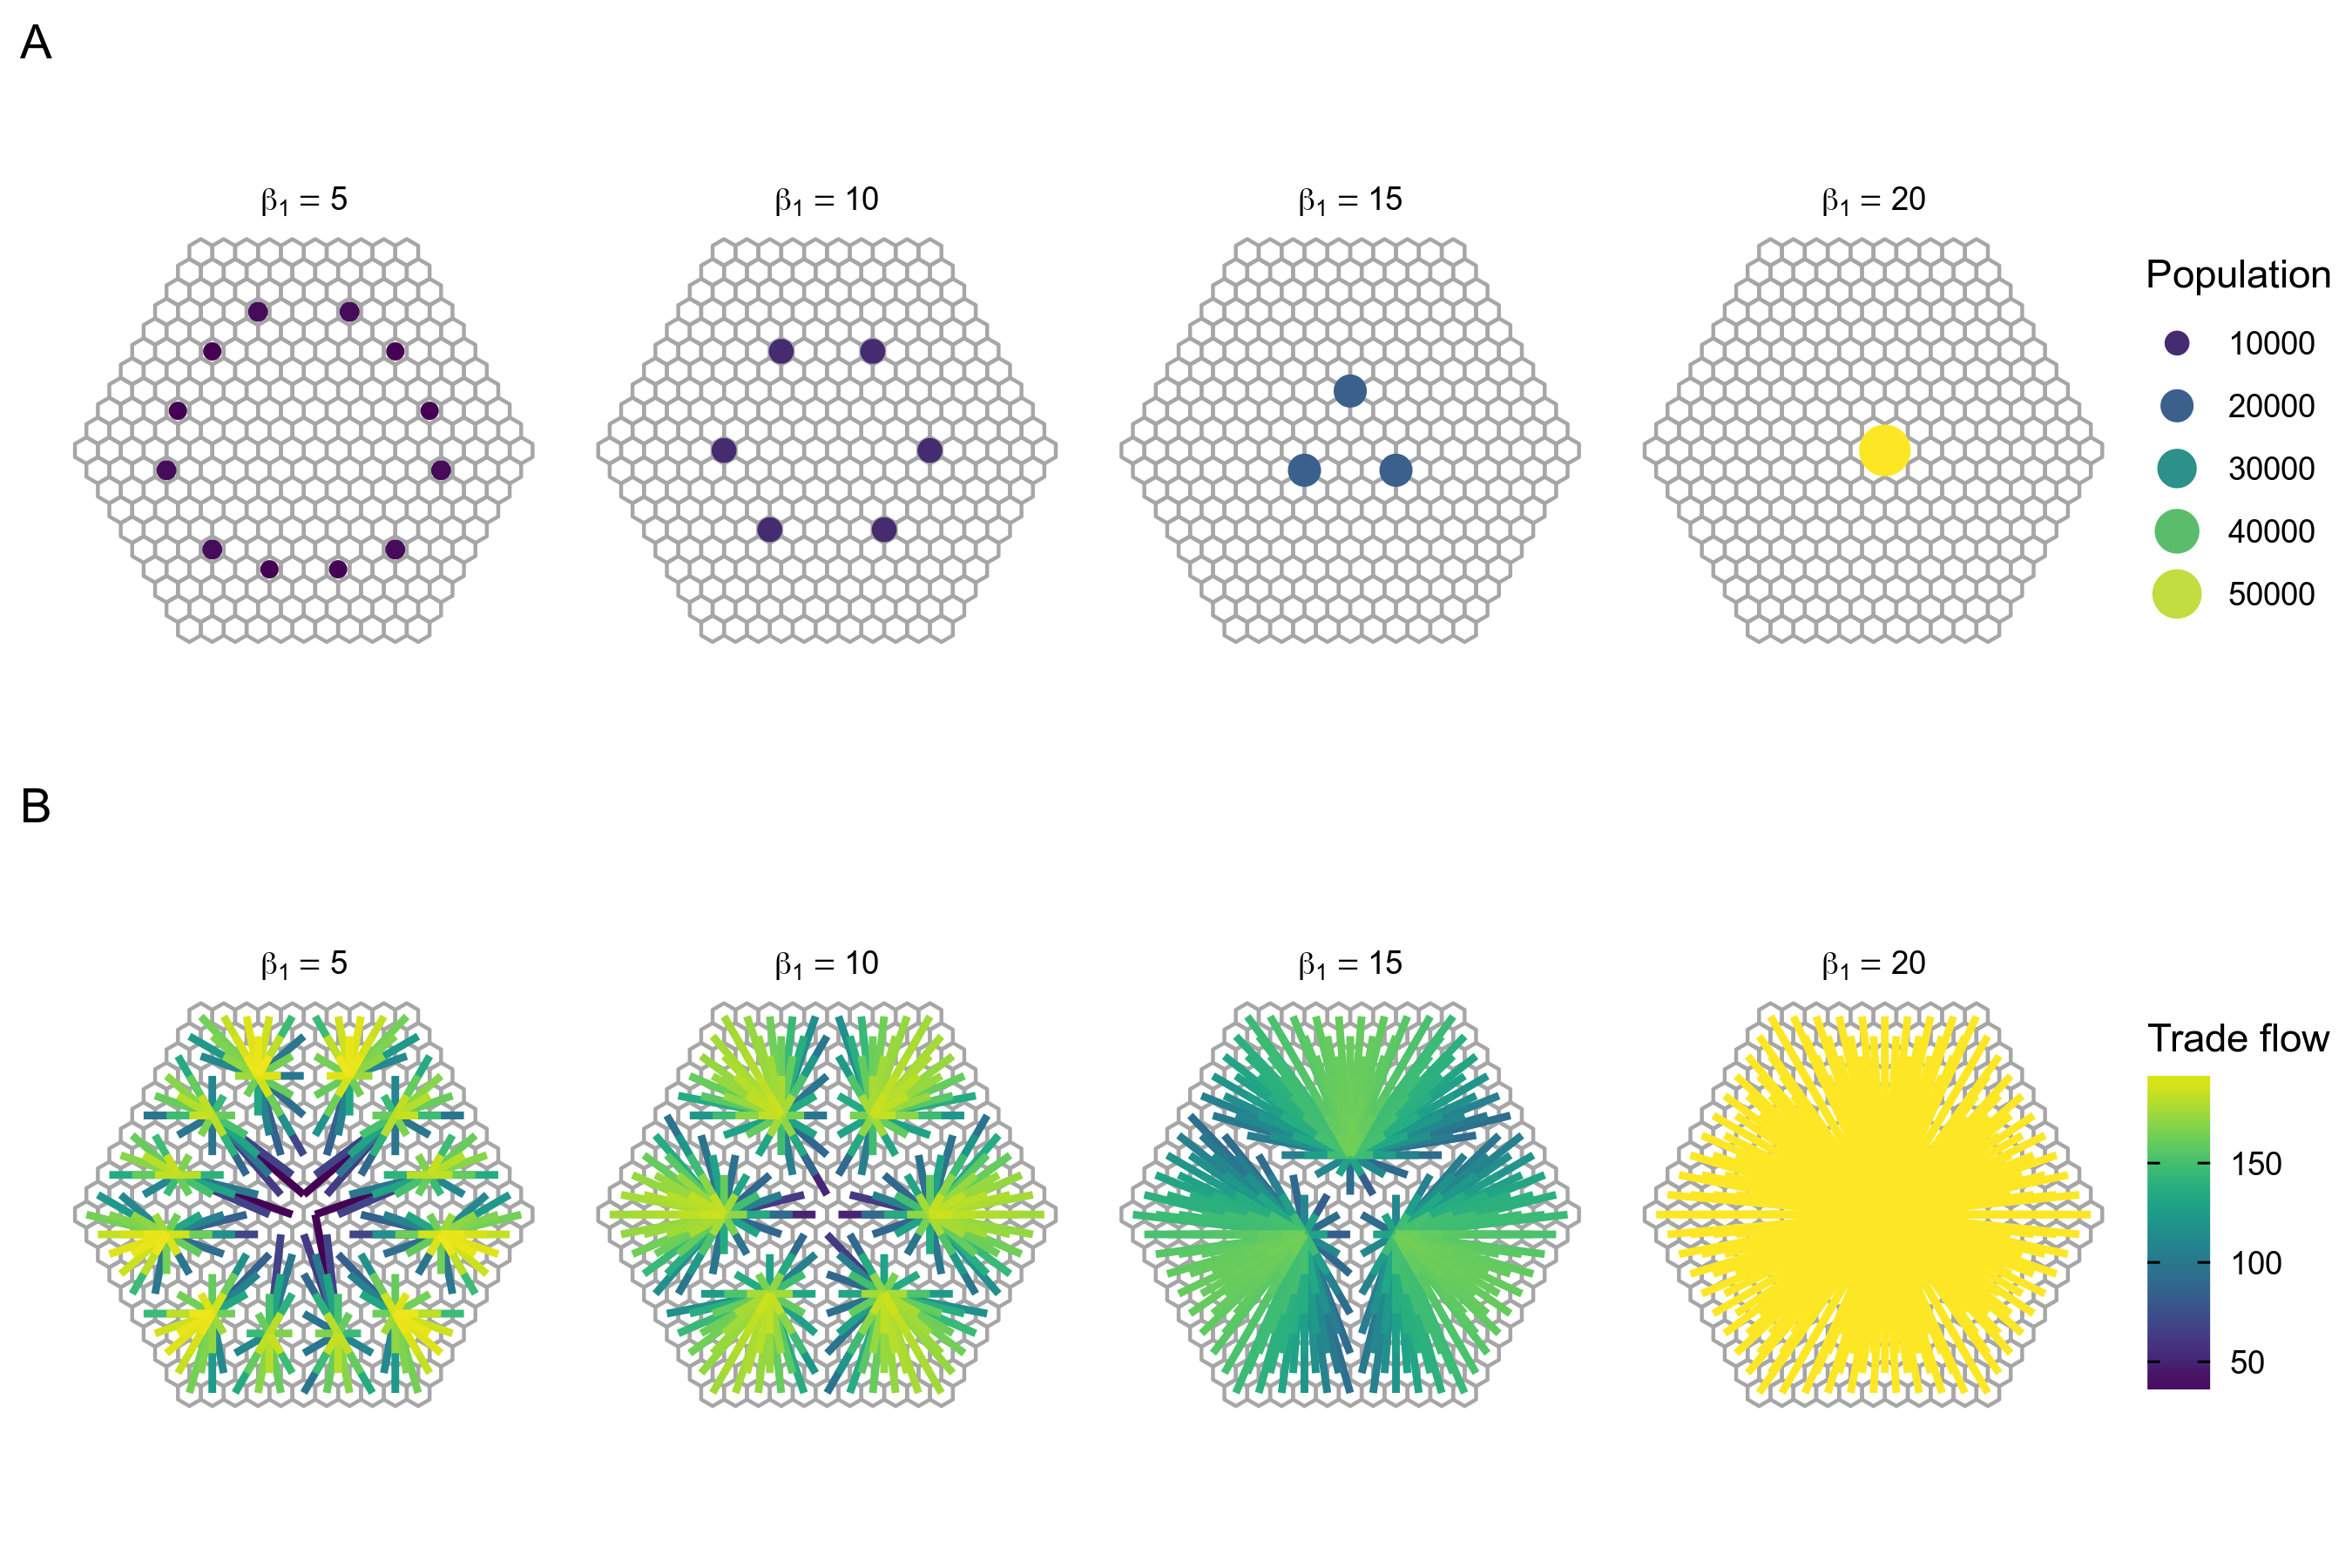
\includegraphics[width = \linewidth]{images/beta1.png}
    \caption[The role of the ease of movement for trade in settlement size and spacing]{The role of the ease of movement for trade in settlement size and spacing. A) Equilibrium settlement patterns and populations for different levels of $\beta_1$, with $\beta_2 = 20, \alpha_1 = 1.15, \alpha_2 = 0$. The $\beta$ parameters are scaled to distance units (here kilometers). B) Same as A, but for each patch an edge is drawn connecting it to the settlement to which the majority of its resources flow. Trade flow is measured in units of food to support 1 person per year.}
    \label{fig:beta1}
\end{figure}


If the costs of moving resources to settlements, as encoded in $\beta_1$, strongly determine the size and spacing of major settlements, what role to the migration costs embedded in $\beta_2$ play? Holding $\beta_1$ constant at a low value (5km) and varying $\beta_2$ allows migrants to move further across the landscape than food resources. The result is a pattern of concentric rings at low values of $\beta_2$ (Figure \ref{fig:beta2}a). When it is difficult to move food over space, migration acts in lieu of food transport by increasing the size of the terminal centers (allowing population to move to populated zones), but this effect and the resulting size of the population is not nearly as strong as that induced by varying $\beta_1$. 

\begin{figure}
    \centering
    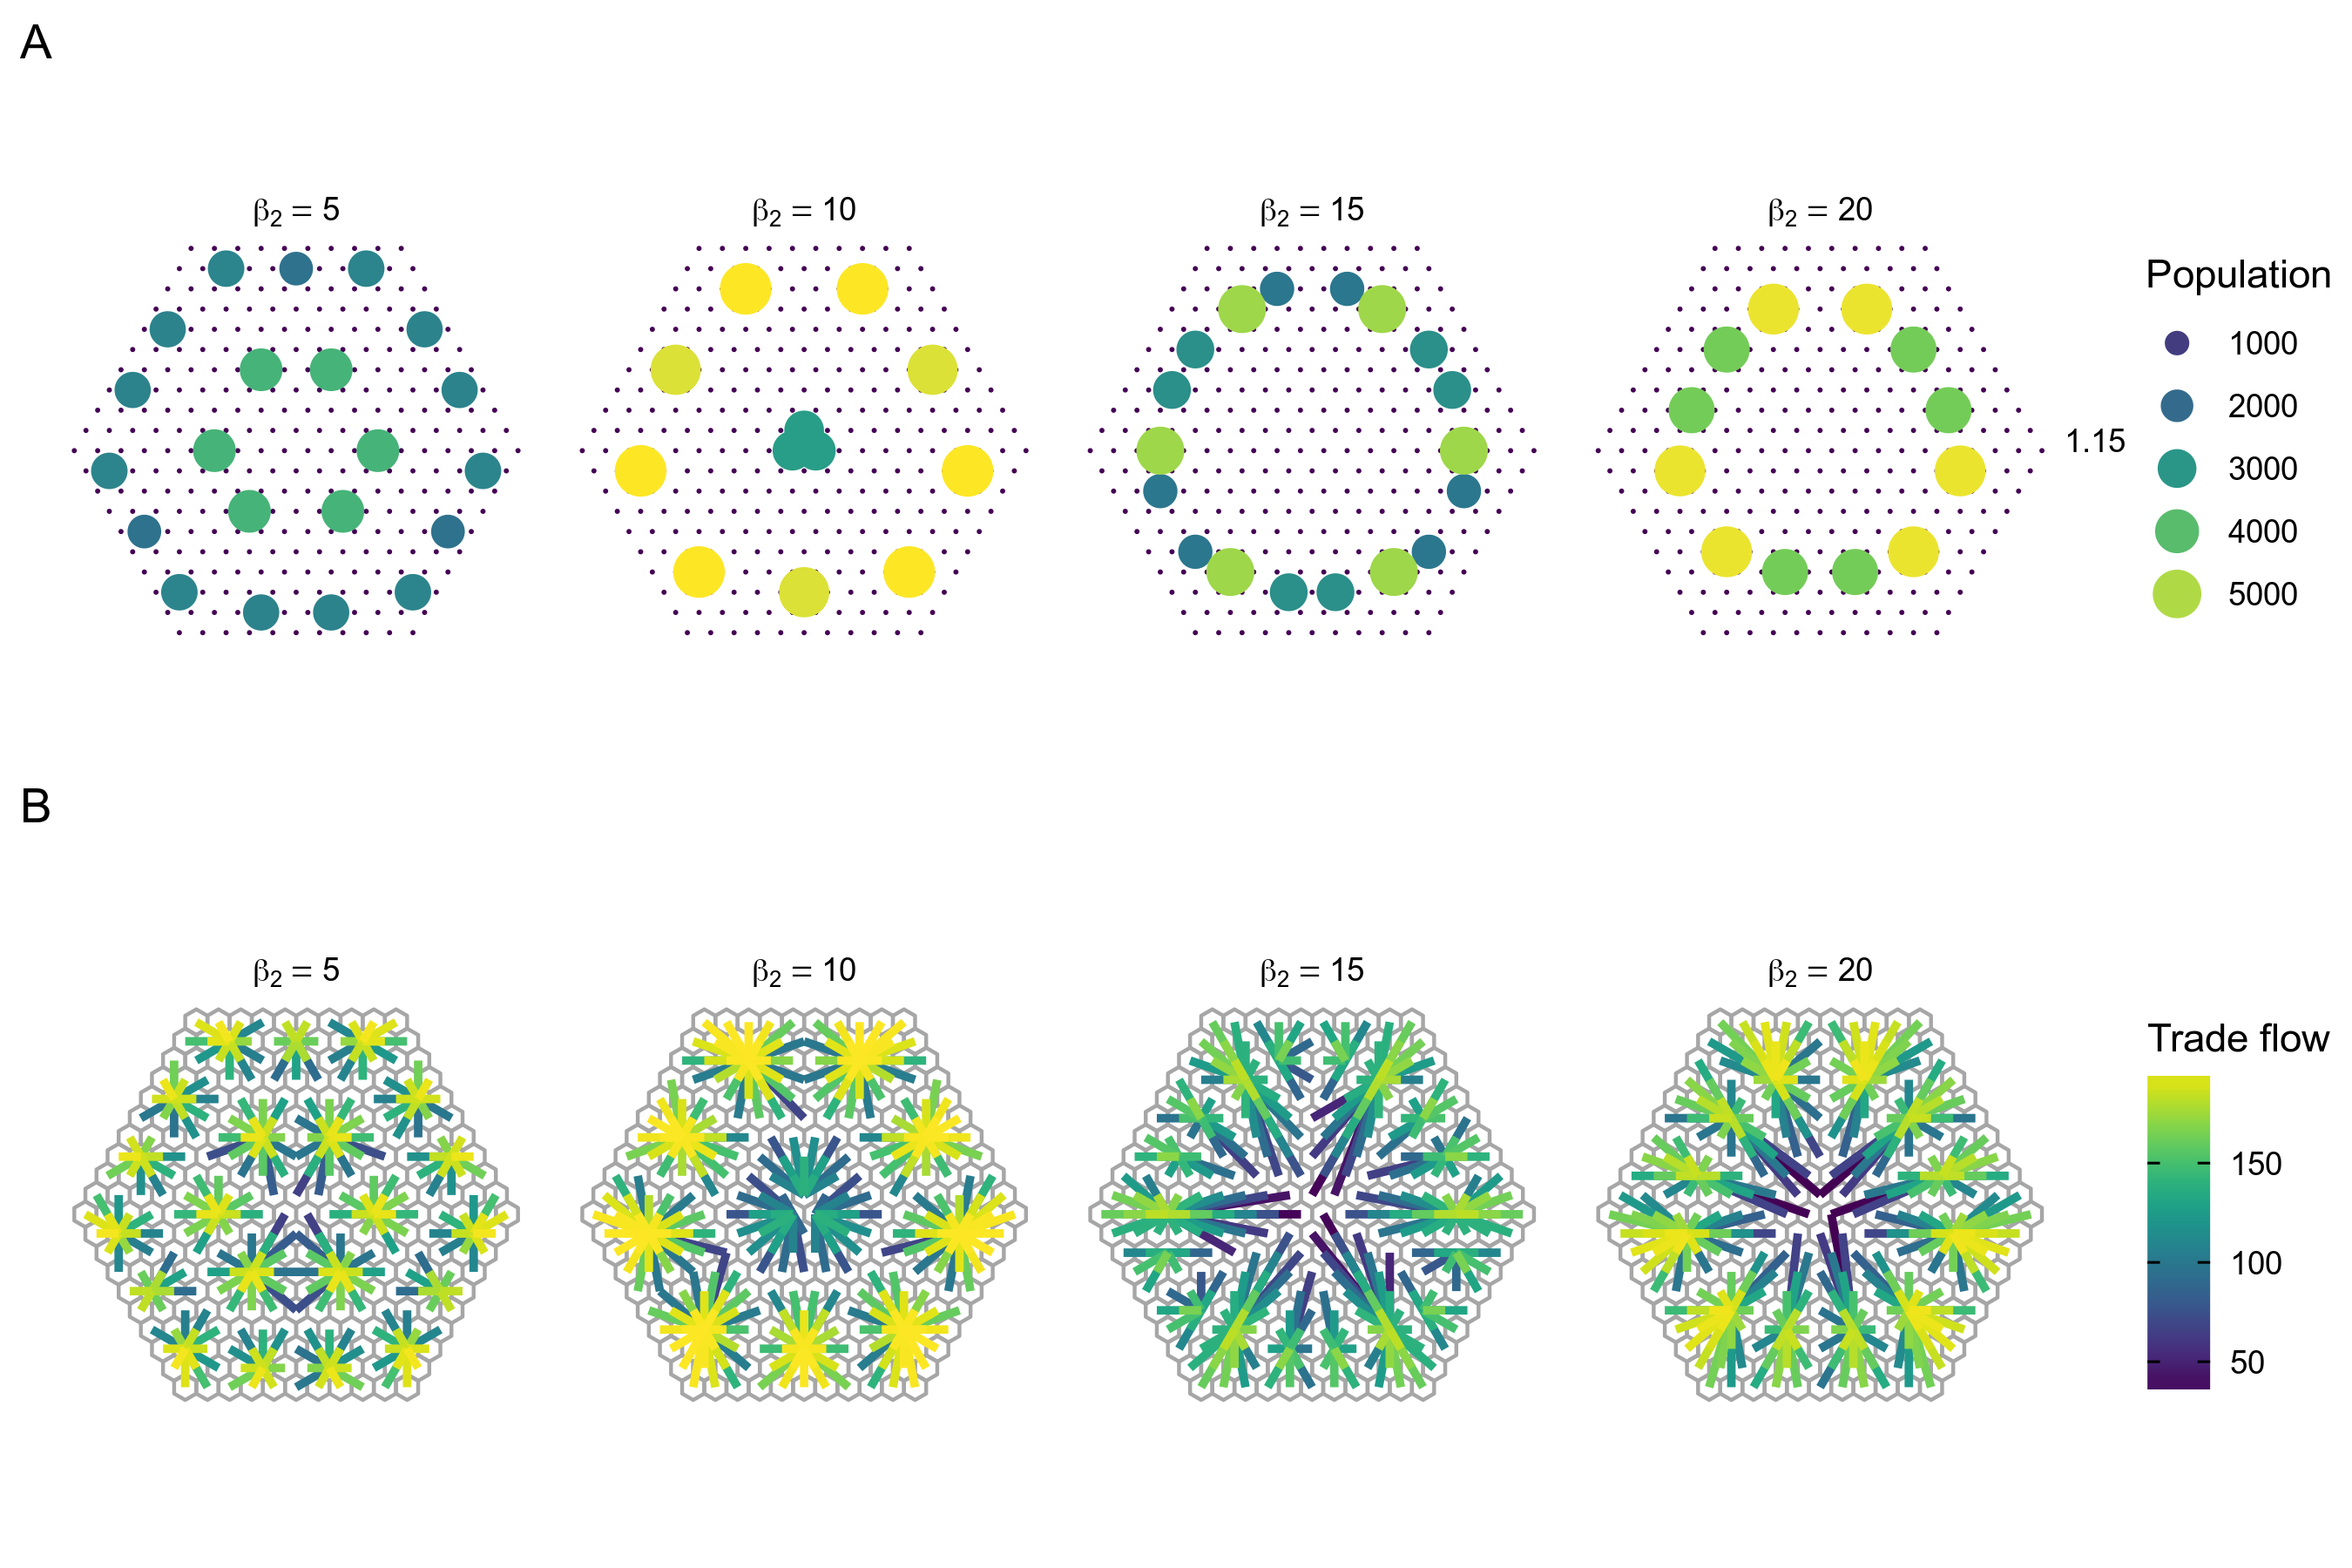
\includegraphics[width = \linewidth]{images/beta2.png}
    \caption[Settlement population (A) and trade flows (B) at equilibrium for different levels of $\beta_2$]{Settlement population (A) and trade flows (B) at equilibrium for different levels of $\beta_2$, the ease of movement for migration, with $\beta_1 = 5, \alpha_1 = 1.15, \alpha_2 = 0$.}
    \label{fig:beta2}
\end{figure}

A settlement's ability to gain an initial surplus because of its position is key to its long-term survival. The absolute productivity of the land is less important than access to resources systems without significant competition from other settlements. Changing $\beta_1$ to facilitate easier resource transport acts to increase the competition between settlements for productive land, making it easier for larger, more distant settlements to out-compete smaller nearby settlements for access to a given resource system. Although the model does not explicitly account for edge effects at the boundary of the spatial domain, in practice the distance scale of spatial interaction encoded in the $\beta$ parameters is much less than the scale of the spatial domain as a whole. That said, the \emph{shape} of the spatial domain does influence the dynamics, as it should in the real world. The initial benefits to a site because of its position in the spatial domain related to other patches leads to increased population growth, which feeds back to allow the settlement to compete for resources and population from sources further afield. 

\subsection{Population-based Migration Increases Settlement Hierarchy; Welfare-based Migration Reduces It}

The parameters $\alpha_1$ and $\alpha_2$ control the relevance of site population and \emph{per capita} welfare in attracting flows of food and migrants. Introducing superlinear scaling parameters to the population size and welfare by increasing $\alpha_1$ and $\alpha_2$ doesn't change the basic interaction between the $\beta$ parameters, but does impact the size hierarchy. Alternately setting $\alpha_2 = 0$ or $\alpha_2 \geq 1$ allows the model to represent scenarios in which only population size determines the attractiveness of a settlement to migrants, or situations in which the balance of population and \emph{per capita} welfare influence migrant decision-making. 

In the first scenario with only population-based migration, there are nonlinear interactions between the migrant attractiveness and ease of movement parameters (Figure \ref{fig:beta2alpha1}). Generally, increasing $\alpha_1$ increases the concentration of populations in fewer centers. As before, the settlements near the edge grow fastest because there is less competition for access to resources. There is a break in this pattern at $\beta_2 \geq 15$ and $\alpha_1 = 1$, where the center becomes filled with multiple settlements of similar size in a hexagon pattern. The number of settlements in this central zone increases with increasing migration. These settlements only extract food from their local resource patch. This core settlement zone is a result of the size and shape of the spatial domain, as at long distance interaction the size and shape of the domain more strongly constrains the possible configurations. These inner zones are only present when $\beta_1$ is low or when $\alpha_1 = 1$, as this zone represents situations where no settlement can get an initial advantage from its location or increasing returns to scale and growth ceases. Settlements at the edge get initial advantages because they have fewer nearby cities competing with them for resources. At low $\beta_2$, this dynamic matters little, but at high $\beta_2$ it sets off a feedback loop as population migrates to the sites with initial advantages. This central zone disappears if $\beta1$ or $\alpha_1$ is increased, allowing for some sites to gain initial advantages that feed forward in time. In these cases, $\beta_2$ no longer changes the broad settlement pattern but rather serves to concentrate more people in fewer, closer core settlements.

\begin{figure}
    \centering
    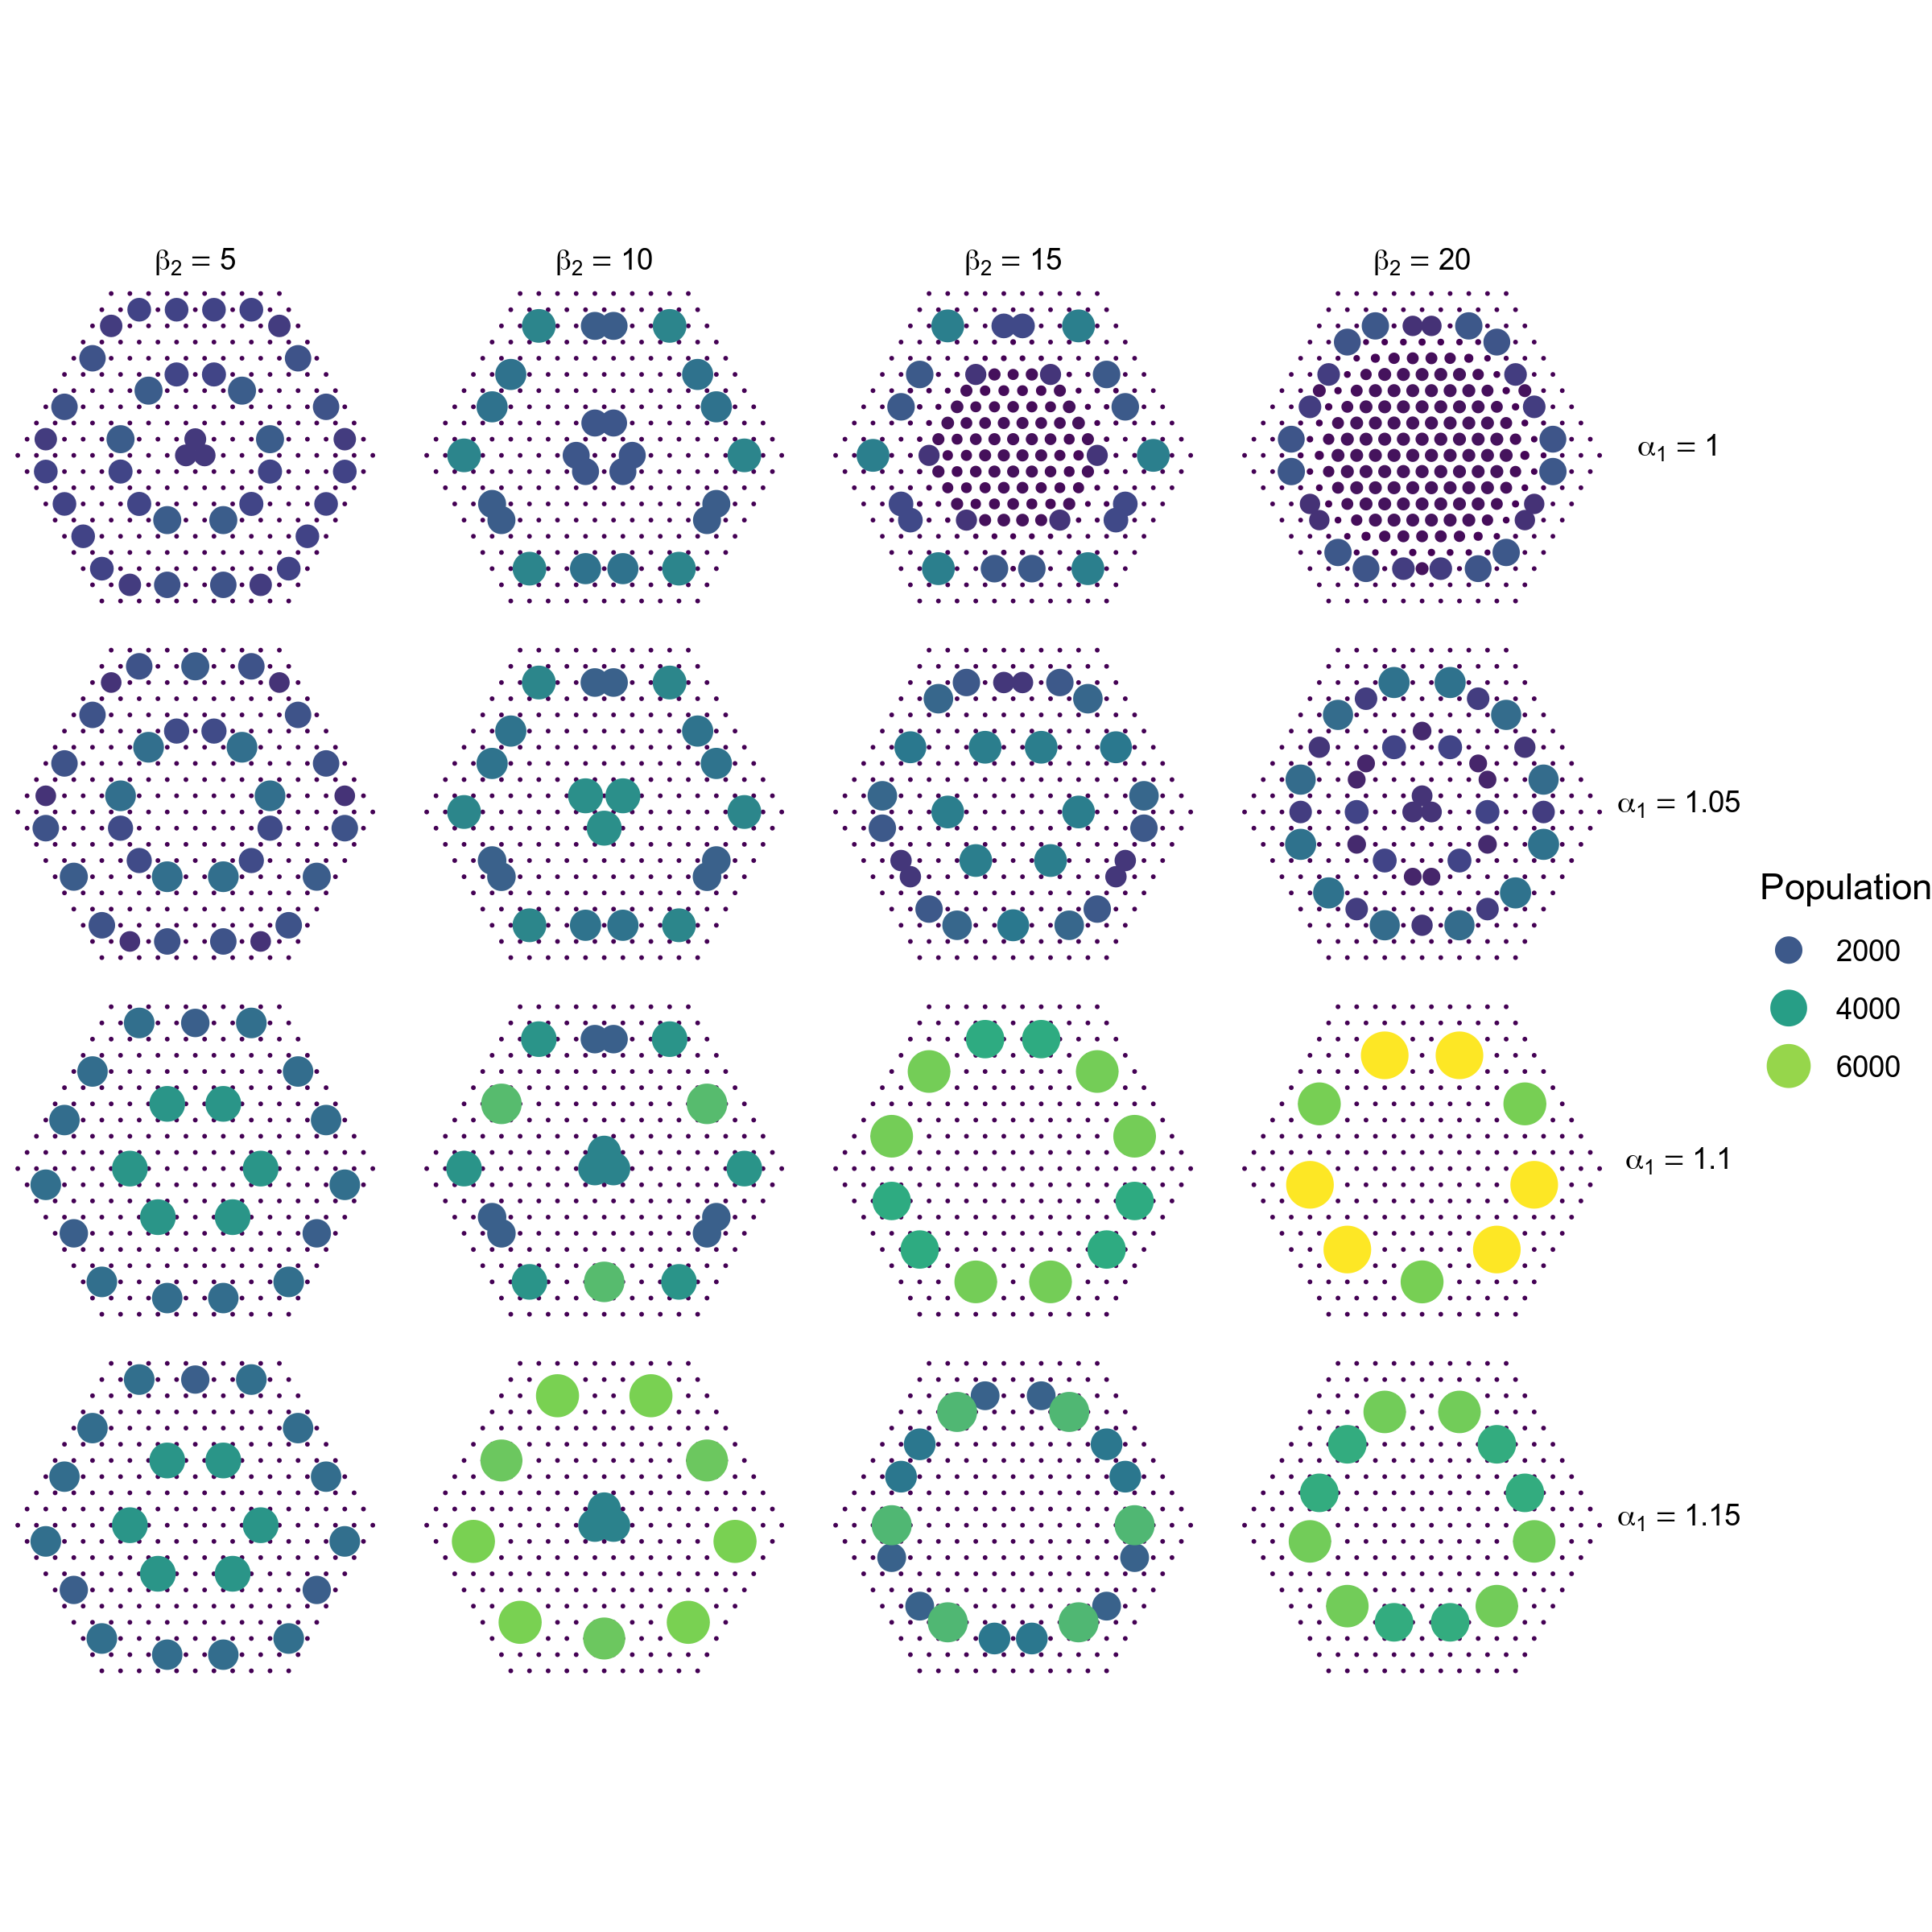
\includegraphics[width = \linewidth]{images/beta2alpha1.png}
    \caption[Interaction between the ease of movement for migrants ($\beta_2$, columns) and the returns to attractiveness for population size ($\alpha_1$, rows)]{Interaction between the ease of movement for migrants ($\beta_2$, columns) and the returns to attractiveness for population size ($\alpha_1$, rows), when the moving food to settlements is difficult and migrants make decisions based only on settlement population size ($\beta_1 = 5$ and $\alpha_2 = 0$). The $\beta$ parameters are scaled to distance units for interpretability, and the $\alpha$ parameters are dimensionless.}
    \label{fig:beta2alpha1}
\end{figure}

Allowing $\alpha_2 \geq 1$, so that people avoid settlements with low welfare, considerably increases the complexity of the system when trade costs are high (Figure \ref{fig:beta2alpha2}). If migrants are attracted to zones with high \emph{per capita} welfare, migration acts to smooth over variations in settlement size due to differential access to resources. The uniform central zone of low population centers discussed earlier arises at even shorter distance migration. This reflects situations where movement is generally easy, but there are few advantages to living in more populated sites so migration acts as a counterbalance to the competition for resources.

\begin{figure}
    \centering
    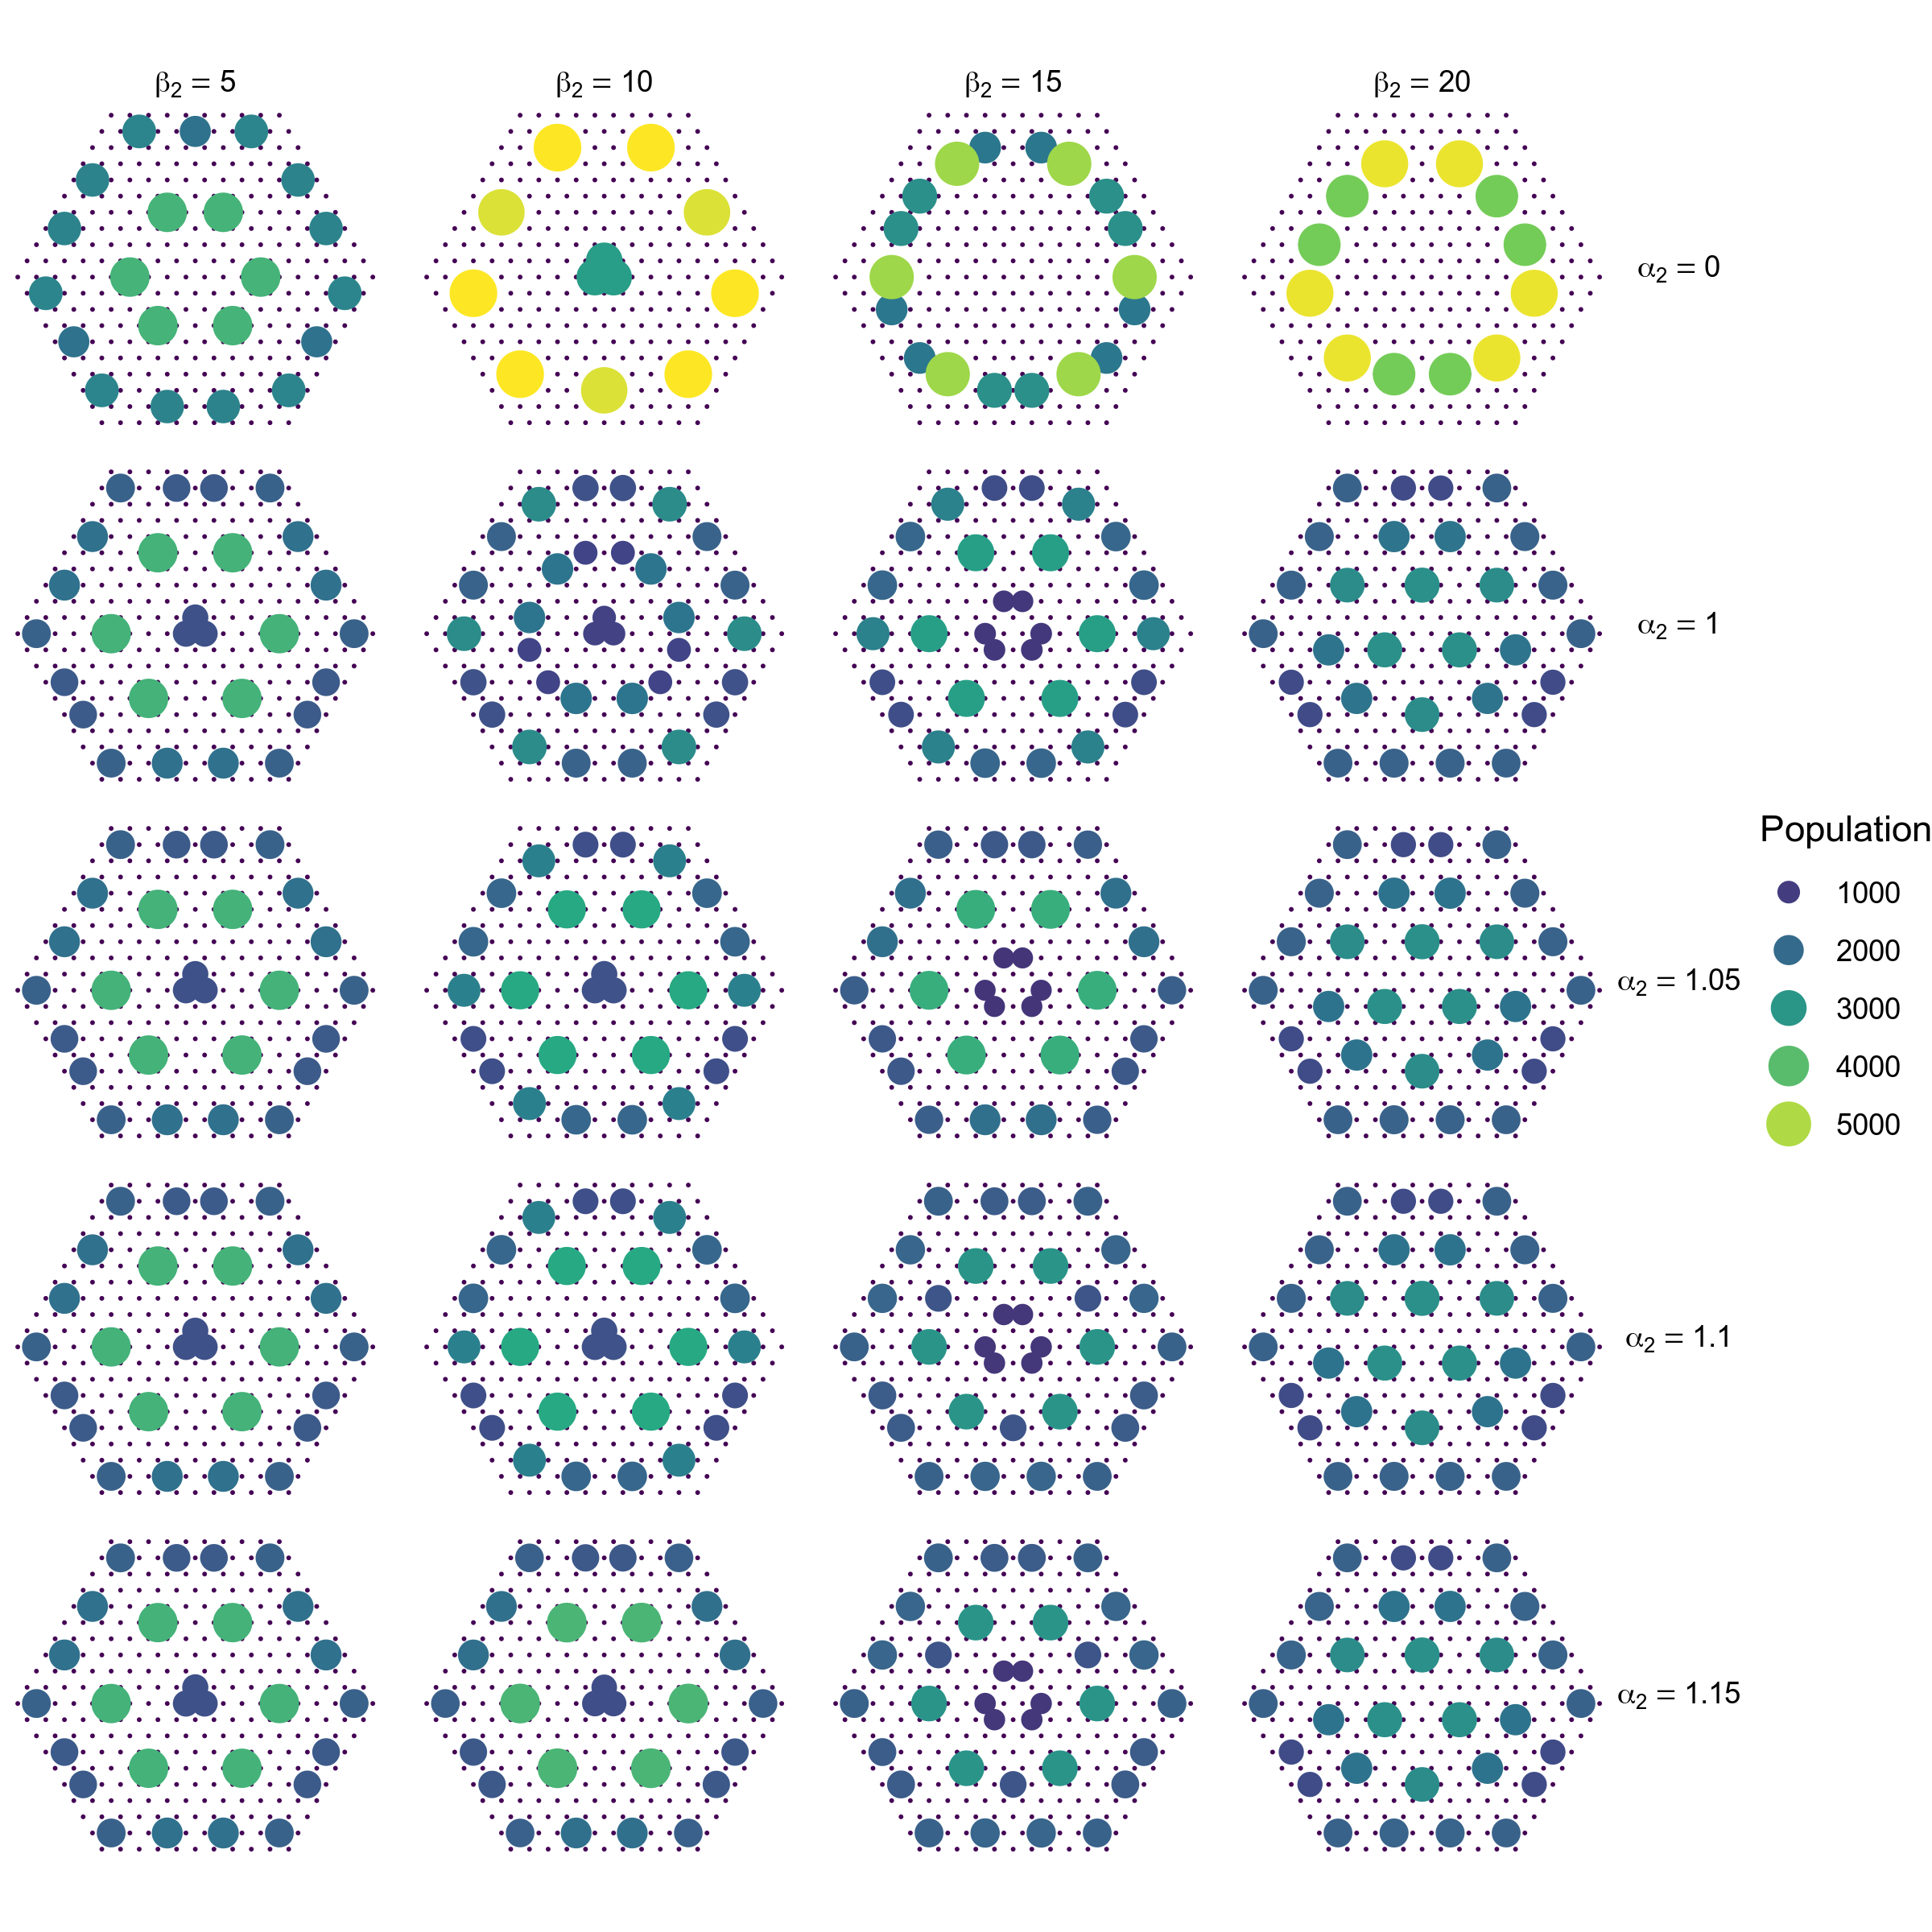
\includegraphics[width = \linewidth]{images/beta2alpha2.png}
    \caption[Interaction between the ease of movement for migrants ($\beta_2$, columns) and the returns to attractiveness for per capita welfare ($\alpha_2$, rows)]{Interaction between the ease of movement for migrants ($\beta_2$, columns) and the returns to attractiveness for \emph{per capita} welfare ($\alpha_2$, rows), when the moving food to settlements is difficult and migrants make decisions based on both settlement population size and \emph{per capita} welfare ($\beta_1 = 5$ and $\alpha_1 = 1.15$).}
    \label{fig:beta2alpha2}
    
\end{figure}

\section{Discussion}

This study sought to explore the relative influence of the costs of transporting food into settlements and the those for moving migrants between them. Analysis of a disaggregated spatial interaction model revealed that trade costs were ultimately more important than migration costs for shaping overall settlement patterns. These results highlight that the precise nature of spatial interaction in a settlement system has important consequences for understanding the development and maintenance of stable settlement patterns in the archaeological record.

The costs of moving resources from resource patches to settlements determine the territorial reach of resource extraction, which is the primary determinant of equilibrium site size and spatial configuration. Even small initial differences in the number of people the local resource patches can support can increase consumption enough to set off a positive feedback between settlement population and resource extraction. The importance of trade flows here is consistent with related modeling efforts that highlight the role of trade networks in extending local carrying capacity in simple consumer resource networks \parencite{Qubbaj2014,Dolfing2019}. 

This dynamic has empirical support. The pattern of 5km settlement-patch modules self-organizing into nucleated settlements harvesting from larger 15-20km ``compound catchments'' with larger settlements thus spaced 30-40km on the landscape has been documented in Bronze Age northern Mesopotamia and Hungary \parencite{Wilkinson1994, Duffy2011SiteSocieties}. These ``compound catchments'' need not themselves be hexagonal. When migration costs are low relative to resource transport, the model predicts fan-shaped compound catchments arising not from centralization around the target settlement but competition with other neighboring settlements, a situation visible in the settlement patterns of central Mexico \parencite{Hirth1978}. In general, it appears that the configuration of resource flows into settlements directly influences the emergent spatial and social structure \parencite{Crabtree2017a}.

The spatial scale of settlement structure in these examples implies the flow of overland food transport attenuates at around 20km, reflecting a value of $\beta_1$ value of 4-5km. This value is supported by analysis of settlement structures across a broad swath of northern Mesopotamia \parencite{Menze2012MappingScale}. Of course this value will vary for different modes of travel, but it provides an appropriate baseline for exploring settlement patterns in other small-scale societies lacking specialized transport technology. An increase in inter-site spacing or the growth of sites in once marginal zones suggests innovations in moving food resources over space, such as the shift from ``hubs'' and ``endogenous upstarts'' to ``exogenous upstarts'' in the settlement history of Mesopotamia with the advent of extensive sheep and goat pastoralism and long-distance trade \parencite{Lawrence2015HubsCrescent, Lawrence2016}.

Migration has a more subtle influence than trade in the model, acting to redistribute population among settlements with less impact on aggregate settlement structure. Migration is most important when food transport costs are particularly high and the territorial reach of small settlements is low. When migrants choose where to travel based on population size alone, the resulting dynamic is one of nucleation and stratification. This phenomenon is ubiquitous in the archaeological record, from the coalescence of Hohokam communities in the US Southwest \parencite{Hill2004}, to Jomon-era Japan \parencite{Crema2013CyclesBay}, and the synoikism of classical Greek \emph{poleis} \parencite{Mackil2004}. Several factors can lead to apparent aggregation and the formation of settlement hierarchy in the archaeological record \parencite{Duffy2011SiteSocieties}, but many are special cases of this population-based dynamic. External threats of warfare or benefits from socio-economic activity may all encourage people to live together, for example, but from an individual's perspective the choice of destination is still made based on population size. 

The ubiquity of nucleation in the archaeological record suggests that the second determinant of migration in the model, \emph{per capita} food supply, is less relevant to migrant decision-making than absolute population. Aggregation in the southern US Southwest is associated with net population decline, for example, as migrants from the north stressed local productive capacity and reduced local welfare \parencite{Hill2004}. Perhaps long-term cycles of dispersion and aggregation, as evidenced in the US Southwest and Jomon-era Japan \parencite{Crema2013CyclesBay}, reflects shifts in the relative importance of absolute population and food supply to population flows. 

An important point that emerges from the archaeological record is the importance of external environmental factors. Settlement aggregation in both the US Southwest and Mesopotamia often occurred in areas with high irrigation potential, or with easy topographic access to other settlements \parencite{Hill2004,Lawrence2016}. Although the model is capable of capturing these influences, this study simulated a regular lattice of settlements overlaying a uniform environment in order to isolate the effects of the spatial interaction on the system's behavior. But the resulting dynamics are nonlinear, which means that the initial and boundary conditions of the settlement system will constrain its ultimate trajectory. In any given real-world setting, the initial distribution of sites, not to mention the spatial configuration of productive land and physical impediments to travel, will influence the resulting settlement patterns. Future explorations of this model should measure the effect of such environmental variability. In particular, this disaggregated modeling framework can help isolate quantitative classes of variability that lead to qualitatively different settlement patterns, such as degrees of spatial or temporal auto-correlation.

Future work should also draw on the extensive toolkit developed in geography and economics for dynamic spatial interaction modeling. Potential methodological innovations include various ways of further disaggregating the ``fast'' flow dynamics or of incorporating more complex or context-specific models into the ``slow'' settlement dynamics \parencite{Fry2012}. For example, how do the costs of transporting resources to settlements interact when the resources include not just food, but other raw materials for energy or craft production that may contribute to a settlement's carrying capacity or attractiveness? Similarly, the migration flows could be disaggregated to explore the interactions between those of different age, ethnic, or social classes \parencite{Altaweel2015}. 

Given more precise models of the spatial flows, the dynamics of settlement growth and decline can also be elaborated. In the present version of the model, the production of food and the production of migrants at each settlement is assumed to be constant or a fixed proportion of population size, respectively. One might instead model the dynamics of the food producers directly, incorporating feedbacks between producer and consumer populations \parencite{Turchin2003}, or allow migration rates to vary based on population size \parencite{Curiel2018} or differences in the levels of \emph{per capita} food consumption \parencite{Anderies2011a}. Even if these elaborations do little to alter settlement patterns at equilibrium, they will introduce important new behaviors as theses systems approach that equilibrium -- the ``transient'' dynamics -- that in concert with variable initial and boundary conditions will be critical for reproducing the complexity visible in the archaeological record.

And it is precisely here, at the interface of archaeological theory and data, where spatial interaction models may contribute most. These models support both dynamical and statistical implementation; the same model can be used as a tool for developing theory from one domain and interpreting data in another. Numerical simulation with these models can help explore the empirical archaeological record, and act as a test bed for the development of new statistical methods. For example, a statistical spatial interaction model estimates only one $\beta$ value, the coefficient of distance in a log-linear regression. How should one interpret this regression coefficient when it is likely that the pattern at hand arose from the interaction of multiple spatial processes? Disaggregated, dynamic spatial interaction models allow researchers to flexibly explore different dynamical processes interacting to form the stable patterns recorded in the field.

This research highlights dynamics \textit{of} networks, not dynamics \textit{on} networks. The approach implicit in many conceptual and mathematical models of networks, and archaeological networks in particular, treats them as static (if nontrivial) structures on which some dynamic of interest plays out. These structures only change in time to the extent that the researcher intervenes by adding or removing nodes and edges manually. This view is understandable given the fragmentary and time-averaged nature of the archaeological record. Instead, the approach used here treats social networks as dynamical systems with continuous flows of matter, information, and energy in constant interaction with their ecological and social environments \parencite{Brughmans2016RomanModelling,Crabtree2015}. Improved representations of social and biophysical dynamics will not only enhance understanding of the empirical settlement patterning in the archaeological record, but will also facilitate future cross-cultural and inter-regional comparisons by providing a shared set of questions and methodological tools for answering them.

Settlement patterns are some of the most basic components of the archaeological record, yet only in recent decades have archaeologists developed the computational expertise and theoretical tools needed to reconstruct the social fabrics binding those settlements together. But the utility of such datasets for addressing questions of societal relevance remains limited. Archaeological settlement pattern data are rarely comprehensible to the researchers, policy advisers, and stakeholders in the developing world most likely to gain meaningful insight from the information they contain. The solution to this problem lies in the fuller integration of theory and data from the broader social sciences. Spatial interaction models can act as a bridge in this respect, allowing archaeologists to leverage decades of accumulated research into the role of space and distance on the societies of the present and the past.

\printbibliography

\end{document}
